\documentclass[tikz,border=2pt]{standalone}
\usetikzlibrary{arrows.meta,automata,positioning}
\usepackage{siunitx}
\definecolor{celadon}{rgb}{0.67, 0.88, 0.69}
\definecolor{lightskyblue}{rgb}{0.61, 0.87, 1.0}
\definecolor{bluebell}{rgb}{0.64, 0.64, 0.82}

\begin{document}
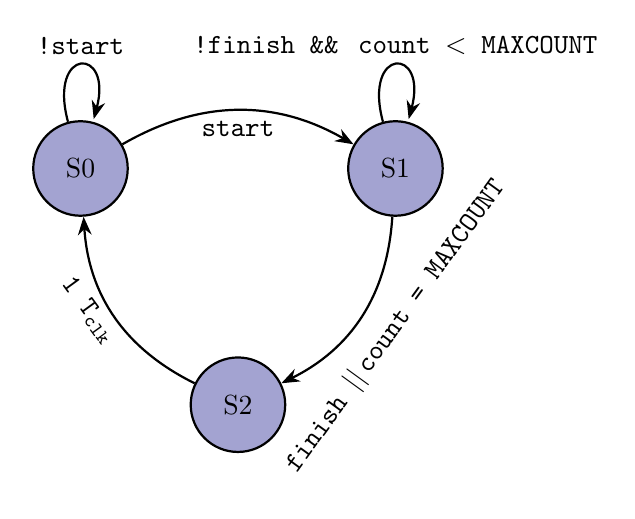
\begin{tikzpicture}[
    >=Stealth,
    every state/.style={
        draw,
        thick,
        circle,
        minimum size=1.2cm,
    },
    every edge/.style={
        draw,
        thick
    }
]

% =====================
% STATI
% =====================
\node[state, fill=bluebell] at (0,0) (S0) {S0};
\node[state, fill=bluebell] at (4,0) (S1) {S1};
\node[state, fill=bluebell] at (2,-3) (S2) {S2};

% =====================
% TRANSIZIONI
% =====================

% S0 -> S1
\path (S0) edge[->, bend left]
node[below]{\texttt{start}}
(S1);

% S1 -> S2
\path (S1) edge[->, bend left]
(S2);

\node[rotate=54] at (4,-2) {\texttt{finish \textbar\textbar \,count = MAXCOUNT}};

% S2 -> S0
\path (S2) edge[->, bend left]
(S0);

\node[rotate=-54] at (0.1,-1.8) {\texttt{1 T$_{\texttt{clk}}$}};

% Loop su S0 (opzionale)
\path (S0) edge[loop above]
node{\texttt{!start}}
(S0);

% Loop su S1 (opzionale)
\path (S1) edge[loop above]
node{\texttt{!finish \&\&\, count $<$ MAXCOUNT}}
(S1);

\end{tikzpicture}
\end{document}